\documentclass[plain,basic]{inVerba-notes}

\newcommand{\userName}{Cullyn Newman}
\newcommand{\class}{BI:\@ 428}
\newcommand{\theTitle}{Pedigree Quiz}
\newcommand{\institution}{Portland State University}

\begin{document}
    \begin{center}
        \hspace{-80 pt}\textbf{1.}\hspace{120pt}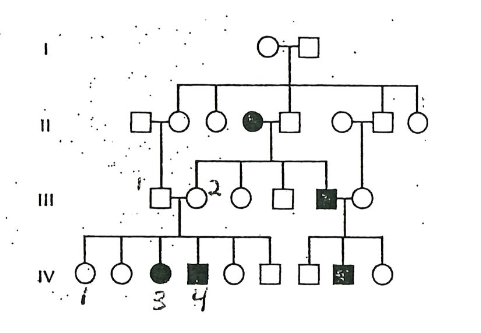
\includegraphics[scale=0.45,angle=0.25,origin=c]{images/pedigree-1.png}
    \end{center}
    \begin{enumerate}[label=\alph*]
        \item Give a mode of inheritance: \textbf{Autosomal recessive (AR)}
        \item Justify why that mode: \textbf{two instances of unaffected individuals having affected offspring, few individuals overall affected.}
        \item Give the genotypes of
        \begin{multicols}{3}
            \begin{enumerate}
                \item[III-1]: \textbf{Aa}
                \item[III-2]: \textbf{Aa}
                \item[IV-1]: \textbf{Aa/AA}
                \item[IV-3]: \textbf{aa}
                \item[IV-4]: \textbf{aa}
            \end{enumerate}
        \end{multicols}
        \item Risk to III 1×2 of having an affected child: \textbf{both are heterozygous, assuming Mendelian: 25\%}
    \end{enumerate}
    \begin{center}
        \hspace{-25pt}\textbf{2.}\hspace{80pt}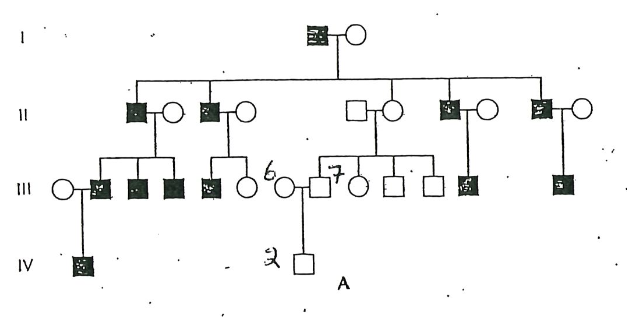
\includegraphics[scale=0.5,angle=-0.5,origin=c]{images/pedigree-2.png}
    \end{center}
    \begin{enumerate}[label=\alph*]
        \item Give a mode of inheritance: \textbf{Y-linked dominant (XD)}
        \item Justify why that mode: \textbf{All affected fathers pass the disease to all sons, no father to daughter transmission}.
        \item Give the genotypes of
        \begin{multicols}{3}
            \begin{enumerate}
                \item[III-6]: \textbf{XX/Xx/xx}
                \item[III-7]: \textbf{yX/yx}
                \item[IV-2]: \textbf{yX,Yx}
            \end{enumerate}
        \end{multicols}
        \item Risk to III 6×7 of having an affected child: \textbf{0\%}
    \end{enumerate}
    \begin{center}
        \hspace{-20pt}\textbf{3.}\hspace{100pt}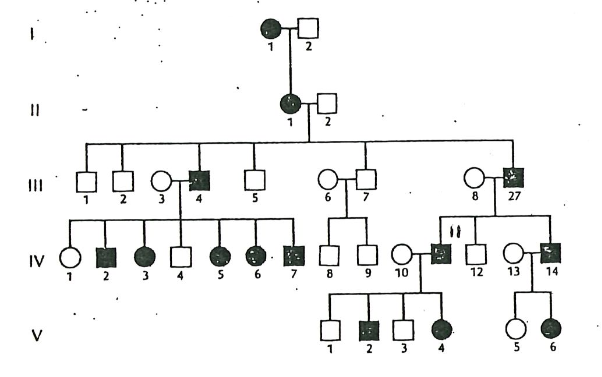
\includegraphics[scale=0.5,angle=-0.5,origin=c]{images/pedigree-3.png}
    \end{center}
    \begin{enumerate}[label=\alph*]
        \item Give a mode of inheritance: \textbf{Autosomal dominant (AD)}
        \item Justify why that mode: \textbf{All affected individuals have a parent that is affected.}
        \item Give the genotypes of
        \begin{multicols}{3}
            \begin{enumerate}
                \item[IV-8]: \textbf{aa}
                \item[IV-10]: \textbf{aa}
                \item[IV-11]: \textbf{Aa}
            \end{enumerate}
        \end{multicols}
        \item Risk to IV 10×11 of having an affected child: \textbf{Aa×aa = 50\%}
    \end{enumerate}
    \begin{center}
        \textbf{4.}\hspace{10pt}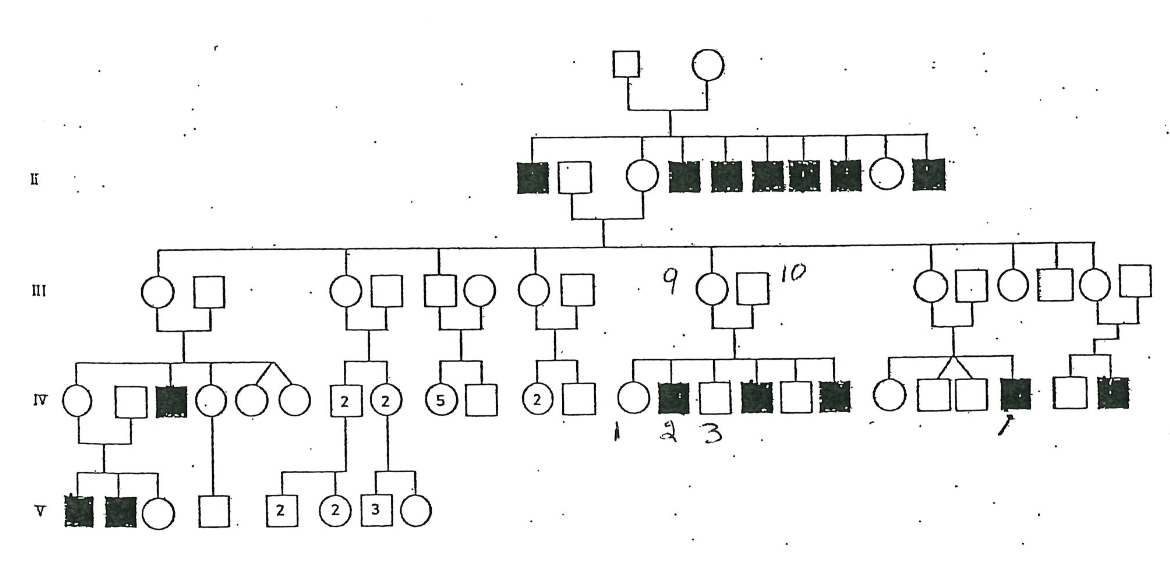
\includegraphics[scale=0.35,angle=-0.15,origin=c]{images/pedigree-4.png}
    \end{center}
    \begin{enumerate}[label=\alph*]
        \item Give a mode of inheritance: \textbf{X-linked recessive (XR)}
        \item Justify why that mode: \textbf{Only males affected, but females can be carriers (and small chance to be affected, but none seen here).}
        \item Give the genotypes of
        \begin{multicols}{3}
            \begin{enumerate}
                \item[III-9]: \textbf{Xx}
                \item[III-10]: \textbf{YX}
                \item[IV-1]: \textbf{Xx/XX}
                \item[IV-2]: \textbf{Yx}
                \item[IV-3]: \textbf{YX}
            \end{enumerate}
        \end{multicols}
        \item Risk to III 9×10 of having an affected child: \textbf{M: 50\% F-carrier: 50\%}
    \end{enumerate}
    \begin{center}
        \textbf{Extra Credit}\qquad\qquad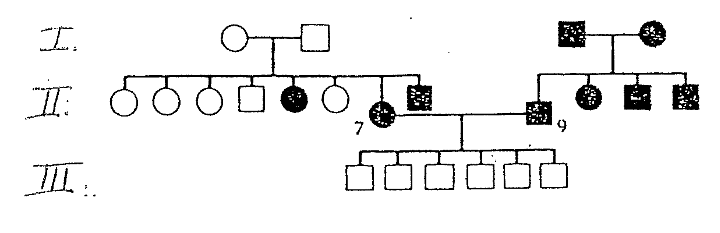
\includegraphics[scale=0.5]{images/pedigree-5.png}
    \end{center}
    \begin{enumerate}[label=\alph*]
        \item Explain this pedigree: \textbf{Due to gene complementation; AAbb×aaBB}.
        \item Genotype of a child in III\@: \textbf{AaBb (carriers)}
    \end{enumerate}

    \textbf{5.} Give the mode of inheritance for the following pedigrees: (Assume the traits are rare)

    \begin{enumerate}[label=\textbf{\alph*}.]
        \item 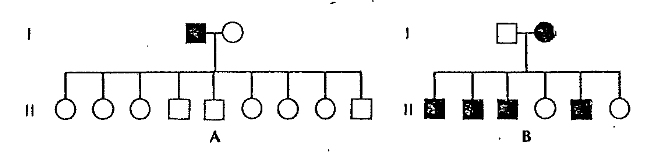
\includegraphics[scale=0.4]{images/pedigree-6.png}
            \begin{itemize}
                \item \textbf{X-linked recessive}
            \end{itemize}
        \item 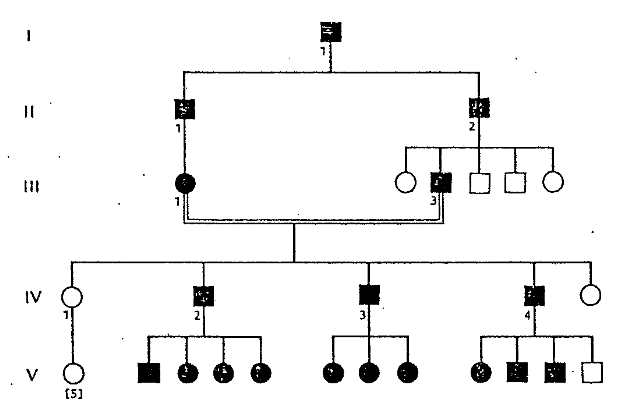
\includegraphics[scale=0.4]{images/pedigree-7.png}
            \begin{itemize}
                \item \textbf{Autosomal dominant}
            \end{itemize}
        \item 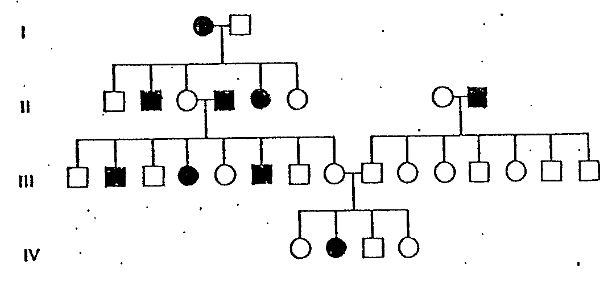
\includegraphics[scale=0.4,angle=-0.5,origin=c]{images/pedigree-8.png}
            \begin{itemize}
                \item \textbf{Autosomal recessive + autosomal dominant}
            \end{itemize}
    \end{enumerate}
\end{document}